\documentclass[aspectratio=169]{beamer}

\graphicspath{{../experiments/exp3_ode_trajectory/results/}}

\usepackage{cmap}
\usepackage[T2A]{fontenc}
\usepackage[utf8]{inputenc}
\usepackage[russian]{babel}
\usepackage{tikz}
\usetikzlibrary{positioning}
\usepackage{array}
\usepackage{multicol}
\usepackage{booktabs}
\usepackage{csquotes}
\usepackage{amssymb,amsfonts,amsmath}

\usecolortheme{beaver}
\usefonttheme[onlymath]{serif}
\setbeamertemplate{navigation symbols}{}
\setbeamertemplate{footline}[page number]
\setbeamertemplate{blocks}[rounded=true,shadow=true]
\setbeamersize{text margin left=0.5cm,text margin right=0.5cm}
\setbeamerfont{author}{size=\normalsize}
\setbeamerfont{institute}{size=\normalsize}
\setbeamerfont{date}{size=\normalsize}
\setbeamerfont{frametitle}{series=\bfseries}
\setbeamertemplate{enumerate item}{\insertenumlabel)}
\setbeamertemplate{enumerate subitem}{\insertenumlabel)}

\title{Геометрический подход к оценке сложности данных на основе генеративных диффузионных моделей}
\author{
    Черноусов Данила\\
    Консультант: Грабовой А.В., к.ф.-м.н.
}
\institute{
    Кафедра интеллектуальных систем, МФТИ
}
\date{2026}

\begin{document}

% ============================================================
% Слайд 1: Титульный лист
% ============================================================
\begin{frame}
    \thispagestyle{empty}
    \maketitle
\end{frame}

% ============================================================
% Слайд 2: Постановка проблемы
% ============================================================
\begin{frame}{Постановка проблемы}
    \begin{block}{Проблема}
        Размер выборки $N$ - плохая оценка сложности
    \end{block}

    \medskip
    \textbf{Хотим:}
    \begin{itemize}
        \item Учитывать связи между объектами
        \item Выполнение ряда свойств
        \item Гипотеза: сложность выборки ограничена сверху
    \end{itemize}

    \medskip
    \begin{block}{Новизна}
        \begin{itemize}
            \item Первая мера сложности учитывающая связи между объектами
            \item Доказанные теоремы позволяют строить произвольные меры
    \end{itemize}
    \end{block}
\end{frame}

% ============================================================
% Слайд 3: Мотивация
% ============================================================
\begin{frame}{Актуальность}
    \textbf{Зачем измерять сложность данных:}
    \begin{itemize}
        \item \textbf{Интерпретируемость} --- предсказание качества модели
              по характеристикам обучающей выборки, а не только по её размеру
        \item \textbf{Активное обучение} --- обучающие батчи с учётом сложности батча
        \item \textbf{Оценка разнообразия} --- сравнение выборок одного размера,
              но разного содержания

    \end{itemize}

\end{frame}


% ============================================================
% Слайд 6: Траекторное вложение
% ============================================================
\begin{frame}{Траекторное вложение}
    \textbf{ОДУ вероятностного потока}:
    \[
        \frac{dz}{dt} = -\dot\sigma(t)\,\sigma(t)\,s(z, t),
        \quad z(0) = x
    \]

    где $s(x,t) = \nabla_x \log p_t(x)$ --- скор-функция 

    \bigskip
    \textbf{Траекторное расстояние:}
    \[
        D(x_i, x_j)^2
        = \int_0^1 \|z_{x_i}(t) - z_{x_j}(t)\|^2\,w(t)\,dt
        = \int_0^1 \|z_{x_i}(t) - z_{x_j}(t)\|^2\,d\mu_w(t)
    \]

    где $w(t) = \mathrm{Beta}(t;\,\alpha,\beta)$ --- плотность вероятности, \;$d\mu_w(t) = w(t)\,dt$ --- индуцированная мера

    \medskip
    $D(x_i, x_j) = \|z_{x_i} - z_{x_j}\|_{L^2([0,1],\,\mu_w;\;\mathbb{R}^D)}$
    
\end{frame}

% ============================================================
% Слайд 7: Мера сложности
% ============================================================
\begin{frame}{Мера сложности}
    \textbf{Гауссово ядро:}\quad
    $K_{ij} = \exp\!\bigl(-\lambda\,D(x_i, x_j)^2\bigr)$,
    \qquad $K_{ii} = 1$, \quad $0 \leq K_{ij} \leq 1$

    \bigskip
    \begin{block}{Сложность выборки}
        \[
            \mathcal{C}(\mathcal{X}) = \log\det(I + K)
            = \sum_{k=1}^{N} \log(1 + \mu_k),
            \quad \mu_k \text{ --- собственные числа } K
        \]
    \end{block}

    \bigskip
    \textbf{Интерпретация:}
    \begin{itemize}
        \item Каждое $\log(1+\mu_k)$ --- вклад одного независимого направления
              в траекторном пространстве
        \item $\mu_k \gg 1$ (новое направление): вклад $\approx \log\mu_k$
        \item $\mu_k \approx 0$ (избыточная точка): вклад $\approx 0$
    \end{itemize}

    \smallskip
    $\mathcal{C}(\mathcal{X})$ --- число независимых семантических
    направлений в данных
\end{frame}

% ============================================================
% Слайд 8: Свойства
% ============================================================
\begin{frame}{Свойства}
    \begin{block}{Теорема}
        Предложенная мера $\mathcal{C}(\mathcal{X}) = \log\det(I+K)$ удовлетворяет:
    \end{block}

    \medskip
    \begin{enumerate}
        \item \textbf{Инвариантность к перестановкам}
        \item \textbf{Липшицевость по выборке}
        \item \textbf{Субаддитивность:}\quad
              $\mathcal{C}(\mathcal{A} \cup \mathcal{B})
              \leq \mathcal{C}(\mathcal{A}) + \mathcal{C}(\mathcal{B})$
        \item \textbf{Ограниченная монотонность:}\quad
              $0 \;<\;
              \mathcal{C}(\mathcal{X} \cup \{x\}) - \mathcal{C}(\mathcal{X})
              \;\leq\; \log 2$
    \end{enumerate}

    \bigskip
    \textbf{Асимптотическое поведение:}
    \begin{itemize}
        \item $N$ одинаковых объектов: $\mathcal{C} \sim \log N$
        \item $N$ различных объектов: $\mathcal{C} \sim N \log 2$
    \end{itemize}
\end{frame}

% ============================================================
% Слайд 9: Эксперимент --- Скорость роста
% ============================================================
\begin{frame}{Эксперимент: скорость роста}
    \begin{columns}[T]
        \begin{column}{0.55\textwidth}
            \begin{figure}
                \centering
                \includegraphics[width=\textwidth]{growth_rate.png}
            \end{figure}
        \end{column}
        \begin{column}{0.42\textwidth}
            \medskip
            Синтетическая смесь гауссиан, $D = 2$, аналитическая скор-функция

            \bigskip
            \begin{itemize}
                \item $N$ кластеров, по 1 точке: $\mathcal{C} \approx N\log 2$
                \item Один кластер, $\sigma = 0.1$: $\mathcal{C} \approx \log(1+N)$
                \item Один кластер, $\sigma = 1$: промежуточный рост
            \end{itemize}
        \end{column}
    \end{columns}
\end{frame}

% ============================================================
% Слайд 10: Эксперимент --- Разделение кластеров
% ============================================================
\begin{frame}{Эксперимент: чувствительность к разделению кластеров}
    \begin{columns}[T]
        \begin{column}{0.55\textwidth}
            \begin{figure}
                \centering
                \includegraphics[width=\textwidth]{varying_separation.png}
            \end{figure}
        \end{column}
        \begin{column}{0.42\textwidth}
            \medskip
            $K = 3$ кластера, $N = 30$ точек, $D = 2$

            \bigskip
            \begin{itemize}
                \item $\mathcal{C}$ растёт с увеличением разделения $\delta$
                \item Выходит на плато при полном разделении кластеров ($\delta \gtrsim 5$)
                \item На плато: $K$ блочно-диагональна
            \end{itemize}
        \end{column}
    \end{columns}
\end{frame}

% ============================================================
% Слайд 11: Эксперимент --- MNIST
% ============================================================
\begin{frame}{Эксперимент: MNIST}
    \begin{columns}[T]
        \begin{column}{0.55\textwidth}
            \begin{figure}
                \centering
                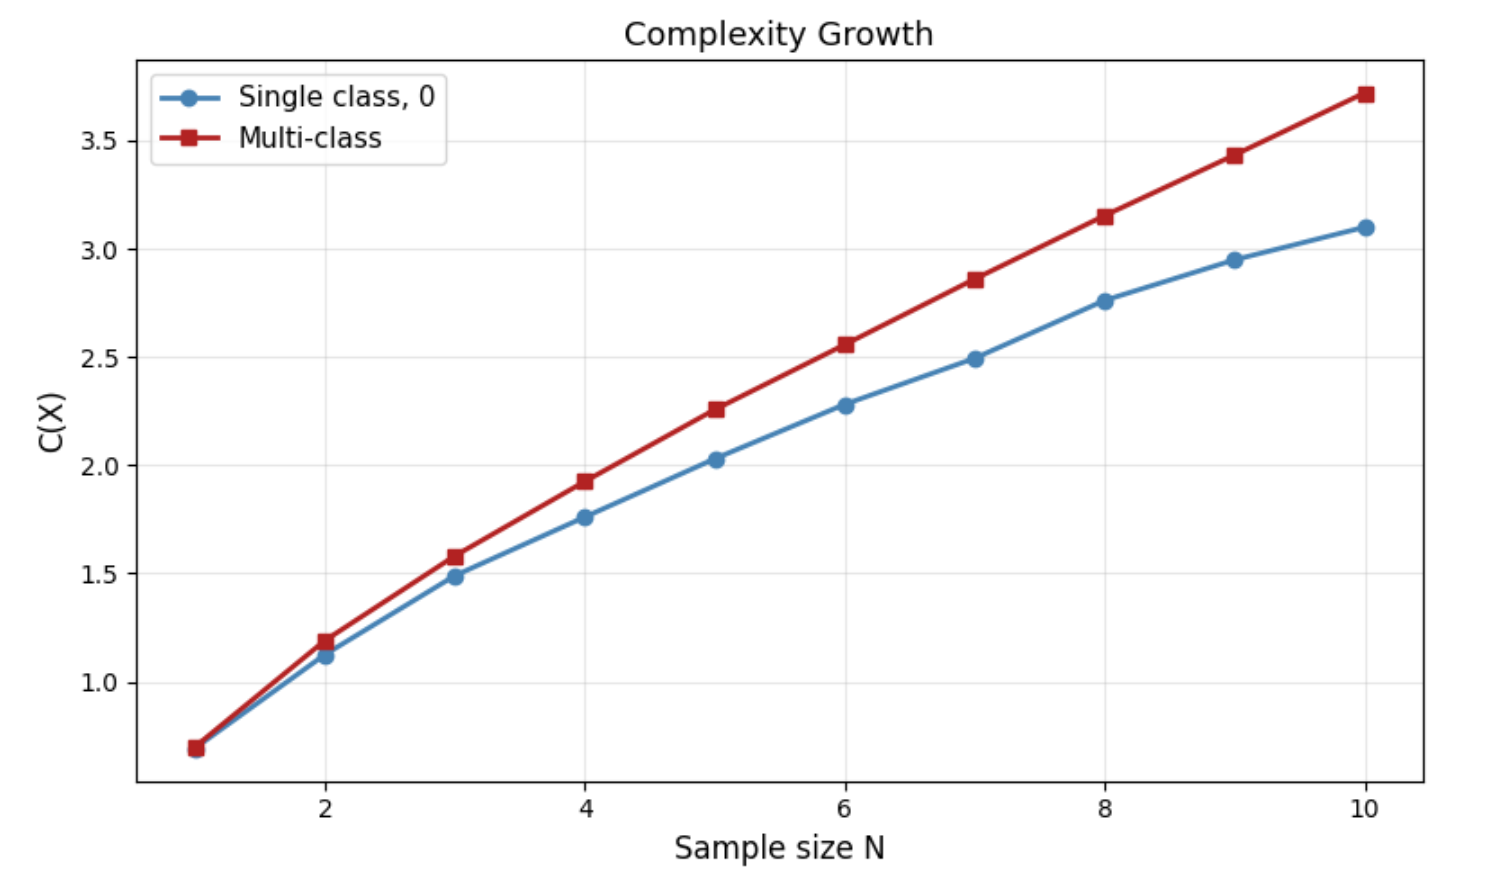
\includegraphics[width=\textwidth]{Mnist_picture.png}
            \end{figure}
        \end{column}
        \begin{column}{0.42\textwidth}
            \medskip
            Предобученная DDPM, ОДУ вероятностного потока

            \bigskip
            \begin{itemize}
                \item Один класс  vs несколько классов
                \item $\mathcal{C}$ мультикласса растёт быстрее
                \item Подтверждает: разнообразные данные $\rightarrow$ большая сложность
            \end{itemize}
        \end{column}
    \end{columns}
\end{frame}

% ============================================================
% Слайд 12: Заключение
% ============================================================
\begin{frame}{Заключение}
    \begin{enumerate}
        \item Определена мера сложности выборки $\mathcal{C}(\mathcal{X}) = \log\det(I+K)$
              на основе траекторных расстояний диффузионной модели
        \item Доказаны ключевые теоремы
        \item Установлена интерпретация с точки зрения дифференциальной геометрии
        \item Проведена экспериментальная проверка на синтетических  и реальных данных
    \end{enumerate}
\end{frame}


\end{document}
